\documentclass[conference]{IEEEtran}
\ifCLASSINFOpdf
   \usepackage[pdftex]{graphicx}
\else
\fi
\usepackage{amsmath}
\usepackage{stfloats}
\hyphenation{op-tical net-works semi-conduc-tor}


\begin{document}
\title{Design of Oversampled ADC Integrators \\ \Large EE240B Project Milestone}
\author{\IEEEauthorblockN{Emily Naviasky}
\IEEEauthorblockA{Department of EECS, UC Berkeley \\enaviasky@berkeley.edu}
\and
\IEEEauthorblockN{Nathaniel Mailoa}
\IEEEauthorblockA{Department of EECS, UC Berkeley \\nmailoa@berkeley.edu}
}
\maketitle

\section{Introduction}

We will propose a design for two integrator stages in an oversampled ADC. The design is driven by some specifications that include input-referred electronic noise, settling time as well as settling accuracy. We have chosen to use the same integrator architecture for both stages but tune the component values for each stage. Section II describes the motivation behind this tuning while Section III provides an early design for the integrator stages.



\section{System Modeling}

To see how our integrators take part in the overall Oversampled ADC architecture, we will first model our integrators with a simple gain and integrator in the z-domain. To model the circuit more accurately, we added two noise sources, one in the input and one at the output. We first assume that the noise in the circuit is white from thermal noise; if the 1/f noise dominates we can modify our circuit to mitigate the issue.

Fig. \ref{integrator-model} shows the system model of our integrator stage. The input noise source $N_{i1}$ for integrator $i$ is caused by the sampling phase $\Phi_1$ of the integrator. Since this sampled noise gets integrated over time, we model it as an addition to the signal at the input. On top of this, we model the noise associated by the amplifying phase $\Phi_2$ by an addition with $N_{i2}$ at the output of the integrator.

\begin{figure}[!h]
\centering
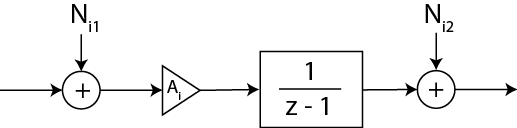
\includegraphics[width=2.5in]{img/integrator-model}
\caption{Integrator model for stage $i$}
\label{integrator-model}
\end{figure}

\begin{figure*}[!b]
\centering
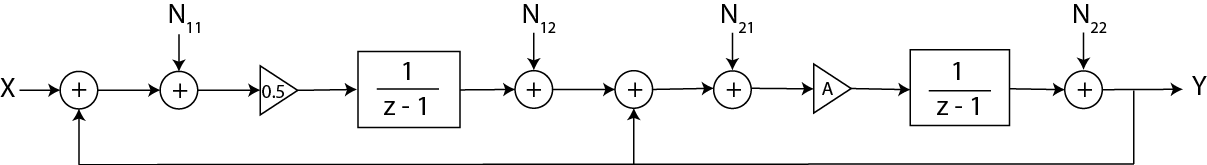
\includegraphics[width=\textwidth]{img/system}
\caption{Oversampled ADC system model}
\label{system-model}
\end{figure*}


Using this model, we can derive the input-referred noise contribution for each of the noise sources. The whole system can be modeled as Fig. \ref{system-model}. Here, the second integrator gain is $A$. We have also modeled the quantizer and DAC as quantization noise $Q$.

From the system model, we can derive how each input affects the output.
\begin{multline}
Y \left( 1 + \frac{A}{z-1} + \frac{A/2}{(z-1)^2}\right) = \\ N_{22} + Q + \frac{A}{z-1}(N_{21}+N_{12}) + \frac{A/2}{(z-1)^2}(N_{11}+X)
\end{multline}

The contribution of each input as seen in the output $Y$ can then be calculated.
$$\frac{Y_X}{X} = \frac{Y_{N11}}{N_{11}} = \frac{A/2}{(z-1)^2+A(z-1)+A/2}$$
$$\frac{Y_{N21}}{N_{21}} = \frac{Y_{N12}}{N_{12}} = \frac{A(z-1)}{(z-1)^2+A(z-1)+A/2}$$
$$\frac{Y_{N22}}{N_{22}} = \frac{Y_Q}{Q} = \frac{(z-1)^2}{(z-1)^2+A(z-1)+A/2}$$

If we divide each expression with the signal transfer function, we get the input-refered contribution of each noise source.
$$N_{11}: 1$$
$$N_{12} = N_{21}: 2(z-1)$$
$$N_{22}: \frac{(z-1)^2}{A/2}$$

\begin{figure}[h]
\centering
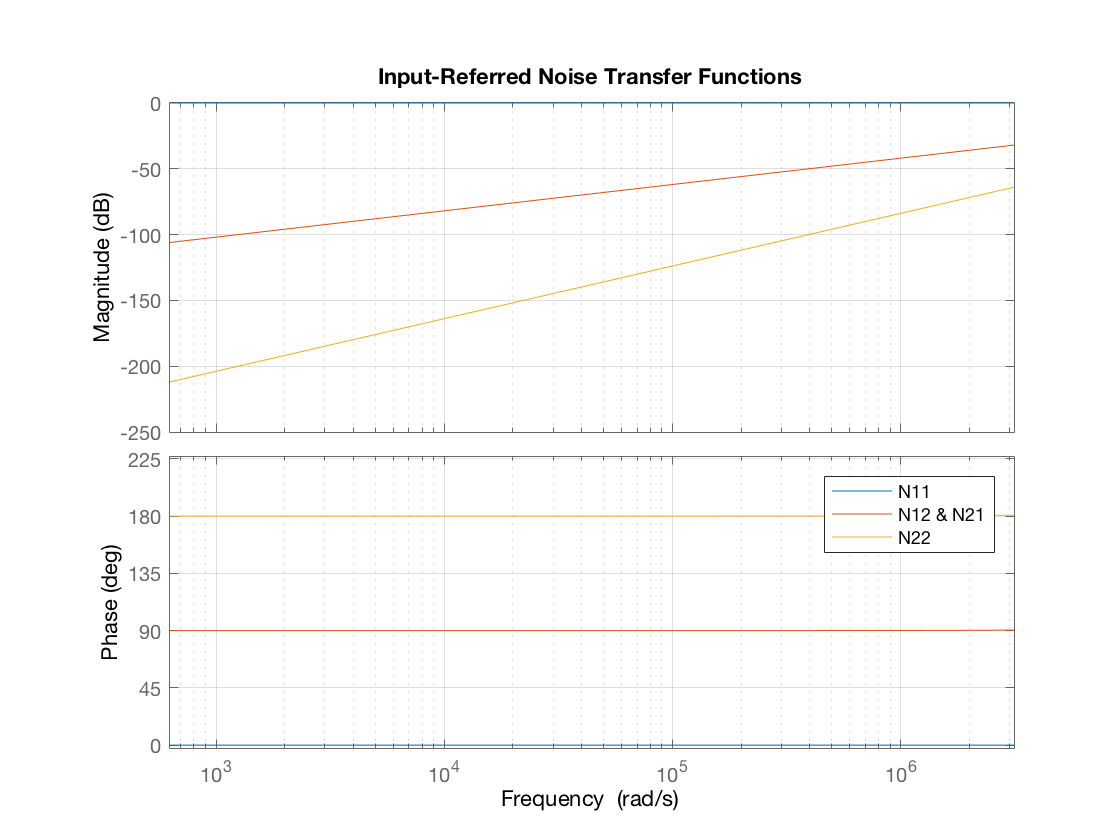
\includegraphics[width=\linewidth]{input-referred-bode}
\caption{Input-referred noise contributions}
\label{noise-tf}
\end{figure}

Fig. \ref{noise-tf} shows the bode plot of these transfer functions in the signal frequencies. As expected, the second integrating stage noise is suppressed more than the first stage and the $\Phi_2$ noise is suppressed more than the $\Phi_1$ noise due to the integrating function of the circuit. When we budget the noise of the circuits, we should take these into account. The first integrator needs to be carefully designed to have a much lower noise compared to the second integrator.

To divide the noise budget, we use a first-order approximation. The $N_{12}$ and $N_{21}$ input-referred transfer function has a highest point at around $-30$dB, so the integrated noise power of these noise sources compared to that of $N_{11}$ is at the worst case $10^{30/10}=1000$ times smaller. Similarly, the noise power contribution of $N_{22}$ is $10^6$ times smaller than that of $N_{11}$.

The second-stage gain $A$ has negligible effects on the input-referred noise contribution, but the larger the gain the smaller the effect of $N_{22}$ and $Q$. In practice this parameter is limited by the signal swing of the circuit.


\section{Design}
For this project the important specifications are:

\begin{center}
\begin{tabular}{|c|c|} 
\hline
Gain (Stage 1) & 0.5 \\
\hline
Input Referred Noise & $10\mu$ $V_{RMS}$ \\
\hline
Settling & 0.1\% in 1.8ns \\
\hline
Sampling Freq & 250M Hz \\
\hline
\end{tabular}
\end{center}

We divided the settling error requirement evenly between static and dynamic error, so $\epsilon_d = 0.05\%$. Furthermore, we decided to budget noise based on the noise factor calculations from the previous section. We see that the noise $\phi_1$ is the most important contribution to the noise. $\phi_2$ will be divided by a factor of 1000, therefore budget nearly all of the noise requirements for noise from $N_{11}$. The spec is for differential noise, so calculating single ended, we need to hit $5\mu$ $V_{RMS}$. We divide that further up, so that there is $3\mu$ $V_{RMS}$ for one input of the first integrator, and $1\mu$ $V_{RMS}$ for one input of the second stage and output of the second stage, taking advantage of the fact that the second integrator can be designed with much looser noise requirements.

From these specifications, we see that the small noise and rapid settling time will require careful design to meet both simultaneously. We began by considering a basic switch cap integrator in fig. \ref{int1} to get an idea of the what values were needed to meet $3\mu$ $V_{RMS}$ per input. We can use a design process similar to that of a sample and hold circuit, with only minor differences due to different switches.

\begin{figure}[h]
\centering
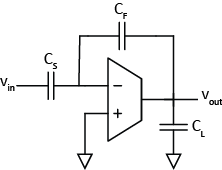
\includegraphics[width=0.4\linewidth]{illustrator/integrator1}
\caption{Basic switched capacitor gain stage}
\label{int1}
\end{figure}

The necessary equations are below. \newline
Gain:
$$\frac{V_{out}}{V_{in}}=\frac{C_S}{C_F}$$
Settling Time:
$$t_s = -\tau ln \left(\epsilon_d \left(1-\beta \frac{C_F}{C_F-C_L}\right)\right)$$
Noise:
$$\phi_1 = \frac{kT}{C_S + C_L}$$
$$\phi_2 = \frac{\alpha}{\beta}\frac{kT}{C_{L,tot}}$$
Where in these equations, beta is the feedback factor. $$\beta = \frac{C_F}{C_S + C_F + C_L}$$ 
In addition, $C_{L,tot}$ is the effective capacitive load.$$C_{L,tot}=C_L+(1-\beta)C_F$$.
And $\tau$ is the time constant of the system. $$\tau = \frac{C_{L,tot}}{(\beta*G_m)}$$

\subsection{First Stage}

We begin by choosing $C_S$ from the noise spec and the equation for $phi_1$. Then $C_F$ is easily obtained from the required gain. We want to meet $3\mu$ $V_{RMS}$ per input, but the BW that we care about noise is only 100-500kHz and our equation for $\phi_1$ is over the entire spectrum. Therefore, we need to divide by the Oversampling Ratio, which is $\frac{f_S}{2BW}$. The noise that we want at the input therefore is $N_{11}=9e-12 V/\sqrt{Hz}$.
%IMPT VALS
$$C_S = 2pF$$ 
$$C_F = 4pF$$
These are somewhat large capacitor values to drive. We next calculate the $G_m$ of the OTA necessary to meet the settling time with those capacitors from $\tau$. We get $G_M = 9mS$, which is a little large, but should be doable with large width MOSFETs.
We began adding parasitics to the transconductor. Parasitic capacitors are from $C_{GS}=\frac{g_m}{\omega_T}$ and we made a first optimistic guess at a conservative $r_o=10k$ and found that in simulation we needed significantly larger $G_M$.
We decided that $G_M$ was getting a little large and decided to check a cascaded setup shown in fig. \ref{int2}. We used ideal transconductors for the diff pairs.

\begin{figure}[h]
\centering
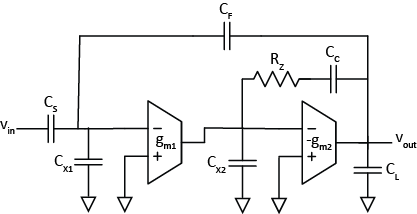
\includegraphics[width=0.7\linewidth]{illustrator/integrator2}
\caption{Cascaded amplifiers with Miller compensation}
\label{int2}
\end{figure}
 
The relevant equations for this part change only a little:
$$\tau = \frac{C_C}{\beta g_{m1}}$$
$$N_{\Phi 2} = \frac{\alpha_1}{\beta} \frac{kT}{C_C} \left( 1+\beta \frac{\alpha_2}{\alpha_1} \frac{C_C}{C_{Ltot}} \right)$$

However, most of the equations for poles and zeros are very approximated, and they do not take into account that the cascaded pair are more stable when $g_{m1}$ is larger than $g_{m2}$. We also had to use a Miller capacitance for pole splitting.

We had to iteratively find a stable value of $g_m$s that met timing, and eventually settled on $g_{m1}=20mS$, $g_{m2}=4mS$.

\begin{figure}[h]
\centering
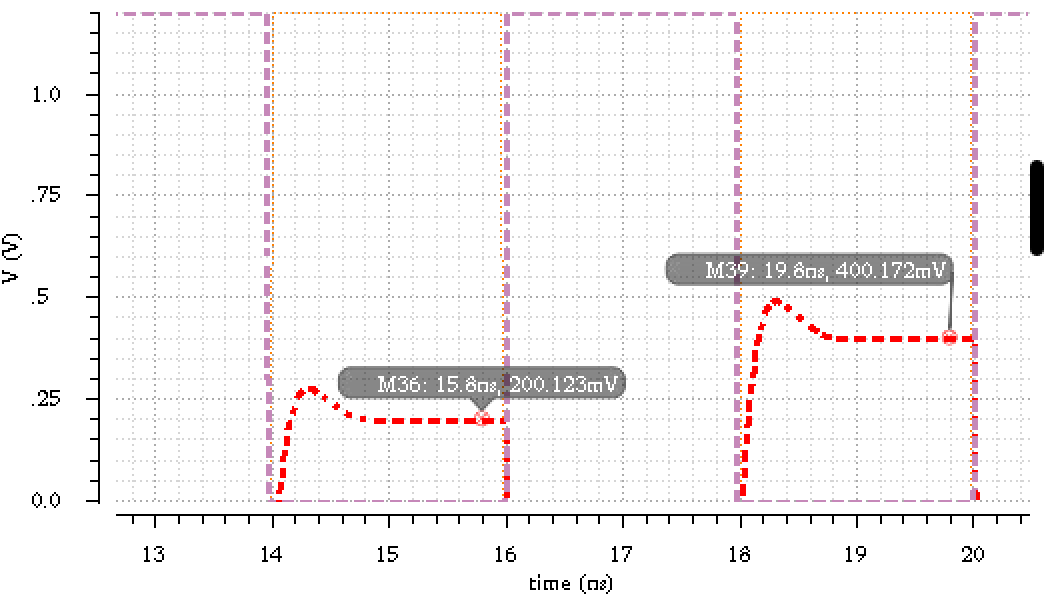
\includegraphics[width=\linewidth]{img/cascaded-tran}
\caption{Transient response of 2-stage amplifier with Miller compensation}
\label{cascaded-tran}
\end{figure}

These value of $g_m$ are not significantly better than the single stage transconductor and the noise of a single stage is better, so we decided that a very large diff pair would be better than cascading.

We re-examined the parasitic resistance and decided that increasing the $r_o$ was the next best option, so that we needed the first stage OTA to be a single stage diff pair with cascoding, and approximated the new $r_o$ as a conservative $100k\Omega$.

We ran a final transient sim to make sure that the settling time of the output of the first stage was 1.8ns to 1\%. 

\begin{figure}[h]
\centering
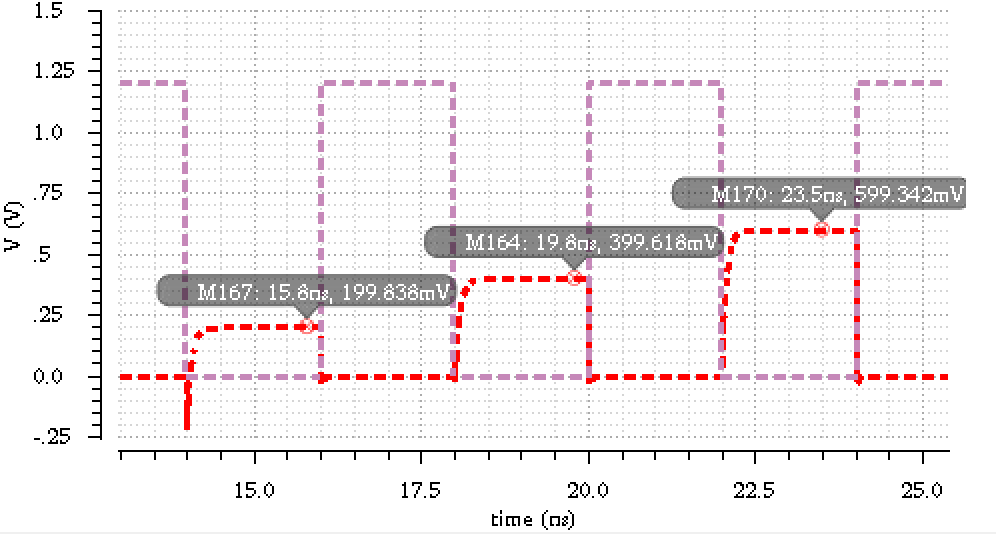
\includegraphics[width=\linewidth]{img/stage1-tran}
\caption{Transient response of first integrator with single-stage amplifier}
\label{stage1-tran}
\end{figure}

The noise simulation was a performed with a noise current source of $\frac{1}{G_m}$ inside of the OTA and $10\Omega$ ON resistances in series with all of the switches. However, PSS and PNOISE are not really meant for integrators so we got the $V/\sqrt{Hz}$ noise density at the output of the integrator which we exported to Matlab, then multiplied by the transfer function from the output to the input, which is $N_{12}$ and then integrated over the BW.

We got a noise of $2.24\mu V_{rms}$ which gives us a lot of room to change the $C_s$ if we need it.

\begin{center}
\begin{tabular}{|c|c|} 
\hline
$C_S$ & 2pF \\
\hline
$C_F$ & 4pF \\
\hline
$G_M$ & 19mS \\
\hline
$R_o$ & 100k \\
\hline
\end{tabular}
\end{center}

In this stage, the most important design factor is meeting the noise requirement. This means that if noise is a problem later in the problem we can increase $C_S$ however, since we are very cleanly meeting the noise spec, we can trade some of it for lower $G_M$ in the gain stage. The large capacitors in the feedback loop relative to the load capacitance of the net stage, however, mean that the loop gain is large and we don't need quite as good of output resistance to correct for 

\subsection{Second Stage}

\begin{center}
\begin{tabular}{|c|c|} 
\hline
$C_S$ & 30fF \\
\hline
$C_F$ & 15fF \\
\hline
$G_M$ & 5mS \\
\hline
$R_o$ & 1M \\
\hline
\end{tabular}
\end{center}

\begin{figure}[h]
\centering
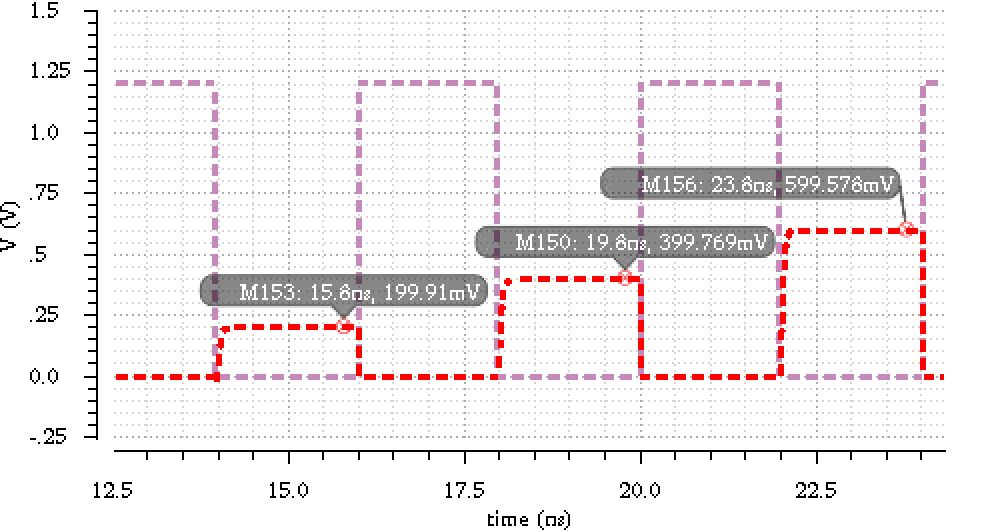
\includegraphics[width=\linewidth]{img/stage2-tran}
\caption{Transient response of second integrator with single-stage amplifier}
\label{stage2-tran}
\end{figure}

\section{Implementation}

gm gonna suck, also, low output impedance sucks too
need cascode or even gain-boosting

RC time constant so suck
need super good switch. gonna be enormous

proposed schematic with all the bells and whistles

use common mode rejection switch on input

offset not a thing in simulation, but here is how we will add it to be through or something

bottom plate sampling with early switches




%\subsection{Subsection Heading Here}
%Subsection text here.


%\subsubsection{Subsubsection Heading Here}
%Subsubsection text here.


% An example of a floating figure using the graphicx package.
% Note that \label must occur AFTER (or within) \caption.
% For figures, \caption should occur after the \includegraphics.
% Note that IEEEtran v1.7 and later has special internal code that
% is designed to preserve the operation of \label within \caption
% even when the captionsoff option is in effect. However, because
% of issues like this, it may be the safest practice to put all your
% \label just after \caption rather than within \caption{}.
%
% Reminder: the "draftcls" or "draftclsnofoot", not "draft", class
% option should be used if it is desired that the figures are to be
% displayed while in draft mode.
%
%\begin{figure}[!t]
%\centering
%\includegraphics[width=2.5in]{myfigure}
% where an .eps filename suffix will be assumed under latex, 
% and a .pdf suffix will be assumed for pdflatex; or what has been declared
% via \DeclareGraphicsExtensions.
%\caption{Simulation results for the network.}
%\label{fig_sim}
%\end{figure}

% Note that the IEEE typically puts floats only at the top, even when this
% results in a large percentage of a column being occupied by floats.


% An example of a double column floating figure using two subfigures.
% (The subfig.sty package must be loaded for this to work.)
% The subfigure \label commands are set within each subfloat command,
% and the \label for the overall figure must come after \caption.
% \hfil is used as a separator to get equal spacing.
% Watch out that the combined width of all the subfigures on a 
% line do not exceed the text width or a line break will occur.
%
%\begin{figure*}[!t]
%\centering
%\subfloat[Case I]{\includegraphics[width=2.5in]{box}%
%\label{fig_first_case}}
%\hfil
%\subfloat[Case II]{\includegraphics[width=2.5in]{box}%
%\label{fig_second_case}}
%\caption{Simulation results for the network.}
%\label{fig_sim}
%\end{figure*}
%
% Note that often IEEE papers with subfigures do not employ subfigure
% captions (using the optional argument to \subfloat[]), but instead will
% reference/describe all of them (a), (b), etc., within the main caption.
% Be aware that for subfig.sty to generate the (a), (b), etc., subfigure
% labels, the optional argument to \subfloat must be present. If a
% subcaption is not desired, just leave its contents blank,
% e.g., \subfloat[].


% An example of a floating table. Note that, for IEEE style tables, the
% \caption command should come BEFORE the table and, given that table
% captions serve much like titles, are usually capitalized except for words
% such as a, an, and, as, at, but, by, for, in, nor, of, on, or, the, to
% and up, which are usually not capitalized unless they are the first or
% last word of the caption. Table text will default to \footnotesize as
% the IEEE normally uses this smaller font for tables.
% The \label must come after \caption as always.
%
%\begin{table}[!t]
%% increase table row spacing, adjust to taste
%\renewcommand{\arraystretch}{1.3}
% if using array.sty, it might be a good idea to tweak the value of
% \extrarowheight as needed to properly center the text within the cells
%\caption{An Example of a Table}
%\label{table_example}
%\centering
%% Some packages, such as MDW tools, offer better commands for making tables
%% than the plain LaTeX2e tabular which is used here.
%\begin{tabular}{|c||c|}
%\hline
%One & Two\\
%\hline
%Three & Four\\
%\hline
%\end{tabular}
%\end{table}


% Note that the IEEE does not put floats in the very first column
% - or typically anywhere on the first page for that matter. Also,
% in-text middle ("here") positioning is typically not used, but it
% is allowed and encouraged for Computer Society conferences (but
% not Computer Society journals). Most IEEE journals/conferences use
% top floats exclusively. 
% Note that, LaTeX2e, unlike IEEE journals/conferences, places
% footnotes above bottom floats. This can be corrected via the
% \fnbelowfloat command of the stfloats package.




\section{Non-Simulation Considerations}



\section{Conclusion}
TODO: The conclusion goes here.




% conference papers do not normally have an appendix


% use section* for acknowledgment
%\section*{Acknowledgment}


%The authors would like to thank...





% trigger a \newpage just before the given reference
% number - used to balance the columns on the last page
% adjust value as needed - may need to be readjusted if
% the document is modified later
%\IEEEtriggeratref{8}
% The "triggered" command can be changed if desired:
%\IEEEtriggercmd{\enlargethispage{-5in}}

% references section

% can use a bibliography generated by BibTeX as a .bbl file
% BibTeX documentation can be easily obtained at:
% http://mirror.ctan.org/biblio/bibtex/contrib/doc/
% The IEEEtran BibTeX style support page is at:
% http://www.michaelshell.org/tex/ieeetran/bibtex/
%\bibliographystyle{IEEEtran}
% argument is your BibTeX string definitions and bibliography database(s)
%\bibliography{IEEEabrv,../bib/paper}
%
% <OR> manually copy in the resultant .bbl file
% set second argument of \begin to the number of references
% (used to reserve space for the reference number labels box)
\begin{thebibliography}{1}

\bibitem{IEEEhowto:kopka}
TODO: H.~Kopka and P.~W. Daly, \emph{A Guide to \LaTeX}, 3rd~ed.\hskip 1em plus
  0.5em minus 0.4em\relax Harlow, England: Addison-Wesley, 1999.

\end{thebibliography}




% that's all folks
\end{document}
